% Patch 0106: TikZ shadings (axial, radial/ball, and a shaded node). Compare with Tectonic's PDF drawn by mutool.
\documentclass{article}
\usepackage{tikz}
\pagestyle{empty}
\begin{document}
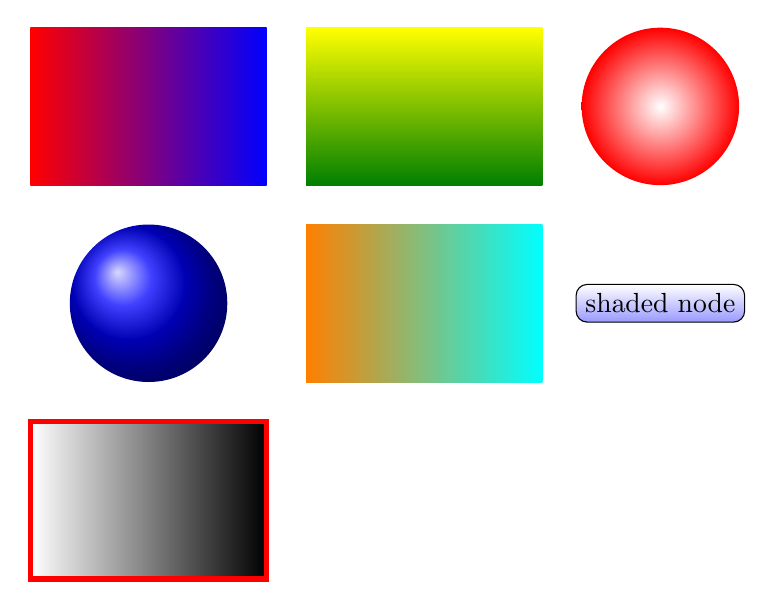
\begin{tikzpicture}
  \shade[left color=red, right color=blue] (0,0) rectangle (3,2);
  \shade[top color=yellow, bottom color=green!50!black] (3.5,0) rectangle (6.5,2);
  \shade[inner color=white, outer color=red] (8,1) circle (1);
  \shade[ball color=blue] (1.5,-1.5) circle (1);
  \shade[shading=axis, shading angle=45, left color=orange, right color=cyan] (3.5,-2.5) rectangle (6.5,-0.5);
  \node[draw, top color=white, bottom color=blue!40, rounded corners] at (8,-1.5) {shaded node};
  \shadedraw[left color=white, right color=black, draw=red, line width=2pt] (0,-5) rectangle (3,-3);
\end{tikzpicture}
\end{document}
